\documentclass{article}
\usepackage[utf8]{inputenc}
\usepackage[T1]{fontenc}
\usepackage[french]{babel}
\usepackage{geometry}
\usepackage{graphicx}
\usepackage[hidelinks]{hyperref}
\usepackage{tocbibind} 

\geometry{a4paper, margin=1in}

\title{Documentation sur le développement}
\date{30/11/2023}
\author{YANG Chen}
\begin{document}

\maketitle
\tableofcontents
\newpage


\section{Besoins du projet}
\subsection{Introduction}
Ce document vise à définir et décrire les besoins de développement de l'application de gestion de portefeuilles financiers. L'application offrira des outils pour créer, gérer et analyser des portefeuilles financiers personnels ou multiples, couvrant les investissements en actions et cryptomonnaies.

\subsection{Besoins Fonctionnels}
\subsubsection{Gestion de Portefeuille}
\begin{itemize}
    \item Création et gestion de portefeuille : Permettre aux utilisateurs de créer et de gérer plusieurs portefeuilles.
    \item Ajout/Suppression d'actifs : Soutenir l'ajout ou la suppression d'actions et de cryptomonnaies dans le portefeuille.
\end{itemize}

\subsubsection{Suivi des Données en Temps Réel}
\begin{itemize}
    \item Suivi de la valeur en temps réel : Afficher en temps réel la valeur de chaque actif dans le portefeuille.
    \item Consultation des données historiques : Fournir une fonction pour consulter la valeur et la performance du portefeuille à des moments passés.
\end{itemize}

\subsubsection{Intégration et Stockage des Données}
\begin{itemize}
    \item Intégration API : Obtenir des données en temps réel des marchés financiers via des API publiques.
    \item Importation de données : Permettre aux utilisateurs d'importer des données de plateformes de transactions externes (comme Coinbase ou Binance).
    \item Cache de données local : Pour améliorer la vitesse et l'efficacité d'accès, stocker les données localement.
\end{itemize}

\subsubsection{Interface Utilisateur}
\begin{itemize}
    \item Interface graphique : Offrir une interface intuitive et facile à utiliser.
    \item Visualisation des données : Présenter les actifs et la valeur du portefeuille sous forme de graphiques.
\end{itemize}

\subsection{Besoins Non Fonctionnels}
\subsubsection{Performance}
\begin{itemize}
    \item Réactivité rapide : Le temps de réponse de l'interface ne doit pas dépasser quelques secondes.
    \item Fréquence de mise à jour des données : La mise à jour des données financières ne devrait pas avoir plus d'une minute de retard.
\end{itemize}

\subsubsection{Sécurité}
\begin{itemize}
    \item Cryptage des données : Les données sensibles doivent être cryptées lors du stockage local.
    \item Sécurité d'accès : Nécessiter un mot de passe utilisateur pour accéder à l'application.
\end{itemize}

\subsection{Fonctionnalités Avancées}
\subsubsection{Fonctions d'Analyse}
\begin{itemize}
    \item Fournir des outils d'analyse de la performance des actifs et des portefeuilles.
    \item Encourager l'innovation et les fonctionnalités d'analyse personnalisées.
\end{itemize}

\subsubsection{Suivi des Transactions}
\begin{itemize}
    \item Suivre les transactions importantes sur la blockchain, en particulier les transactions de grande valeur (connues sous le nom de "traque des baleines").
\end{itemize}

\subsubsection{Choix de la Devise}
\begin{itemize}
    \item Permettre aux utilisateurs de choisir la devise de référence pour afficher la valeur des actifs (par exemple, EUR, USD, etc.).
\end{itemize}

\subsection{Besoins de l'Interface Utilisateur}
\begin{itemize}
    \item Intuitivité : L'interface doit être intuitive et facile à comprendre, simplifiant l'opération pour l'utilisateur.
    \item Personnalisation : Offrir une certaine mesure de personnalisation de l'interface et des options fonctionnelles.
\end{itemize}

\subsection{Contraintes Système}
\begin{itemize}
    \item Limitations techniques : L'application doit être compatible avec les systèmes d'exploitation et dispositifs principaux.
    \item Conformité légale : Respecter les lois et réglementations relatives aux données financières et à la vie privée.
\end{itemize}

\subsection{Spécification Du Code}
\begin{itemize}
    \item Langage de programmation : Java
    \item Style de codage 
    \subitem Suivez les conventions de code Java d'Oracle
    \subitem Utilisez une indentation appropriée (généralement quatre espaces)
    \item Structure du projet
    \subitem Suivez la structure standard des projets Maven
    \subitem Le code source est placé dans src/main/java et le code de test dans src/test/java
    \item Conventions de dénomination
    \subitem Les noms de classes et d'interfaces sont nommés en CamelCase
    \subitem Les noms de méthodes et de variables sont nommés en camelCase
    \subitem Les constantes sont séparées par des lettres majuscules et des traits de soulignement (par exemple, MAX\_VALUE)
    \item Spécification des annotations
    \subitem Utilisez Javadoc pour annoter les classes, les méthodes et les champs publics
    \subitem Utilisez des commentaires de ligne pour les segments de code logiques complexes
    \item Gestion des erreurs
    \subitem Préférez la gestion des exceptions au renvoi de codes d'erreur
    \subitem Les exceptions personnalisées doivent être claires et significatives
    \subitem Évitez les blocs catch vides
    \item Meilleures pratiques en matière de performances
    \subitem Évitez de créer des objets inutiles dans les boucles
    \subitem Utilisez des structures de données appropriées
    \subitem Optimisez les interactions avec les bases de données et les appels au réseau
    \item Spécification des tests
    \subitem Écrivez des tests unitaires qui couvrent les principales fonctionnalités et les conditions limites
    \subitem Utilisez JUnit ou d'autres cadres de test
    \item Contrôle de version
    \subitem Gérez le code à l'aide d'un système de contrôle de version tel que Github
    \subitem Suivez un processus clair de gestion des branches et de demande de fusion
\end{itemize}
\section{Méthodologie de développement et gestion de projet}

\subsection{Choix du modèle en cascade}

Ce projet utilise le modèle en cascade comme méthodologie de développement logiciel. Le modèle en cascade est une méthode de développement séquentielle où chaque phase doit être complètement terminée avant de passer à la suivante. Ce modèle convient aux projets avec des objectifs clairs et des exigences stables.

Bien que notre équipe soit petite, composée de seulement deux membres, le choix du modèle en cascade est le plus approprié pour plusieurs raisons :
\begin{itemize}
    \item \textbf{Objectifs clairs du projet} : Les objectifs et les besoins du logiciel sont bien définis au début du projet.
    \item \textbf{Expérience des membres} : C'est la première participation de notre membre Remi à un projet Java, donc une approche structurée et phasée aidera à une meilleure compréhension et participation.
\end{itemize}

\subsection{Planification du projet et chronologie}

Voici le plan détaillé du projet et la chronologie prévue :

\begin{itemize}
    \item \textbf{26 novembre 2023} - Lancement du projet
    \begin{itemize}
        \item Définition des objectifs et des exigences du projet.
        \item Discussion et détermination de la conception et de l'architecture de base du logiciel.
    \end{itemize}

    \item \textbf{1er décembre 2023} - Préparatifs initiaux
    \begin{itemize}
        \item Finalisation du document de besoins.
        \item Conception de l'architecture logicielle.
        \item Création de la structure du projet.
        \item Réalisation des diagrammes UML et des flux de processus métier.
    \end{itemize}

    \item \textbf{3 au 7 décembre 2023} - Création de classes et itération de la documentation
    \begin{itemize}
        \item Création de toutes les classes nécessaires selon le diagramme UML.
        \item Première itération de l'ensemble du document de développement pour assurer l'exactitude et l'exhaustivité de toutes les informations.
    \end{itemize}

    \item \textbf{10 au 14 décembre 2023} - Intégration et tests de l'API
    \begin{itemize}
        \item Finalisation de l'intégration avec les API externes.
        \item Réalisation de tests fonctionnels pour assurer la correcte intégration et la stabilité de l'API.
    \end{itemize}

    \item \textbf{17 au 22 décembre 2023} - Développement de la base de données et du frontend
    \begin{itemize}
        \item Construction de la base de données.
        \item Début du développement du frontend en JavaFx.
        \item Commencement du développement du backend.
        \item Deuxième itération du document de développement.
    \end{itemize}

    \item \textbf{25 décembre 2023 au 6 janvier 2024} - Développement du backend et tests
    \begin{itemize}
        \item Finalisation du développement du backend.
        \item Début des tests sur l'ensemble du système, incluant les tests unitaires et d'intégration.
    \end{itemize}

    \item \textbf{8 au 12 janvier 2024} - Finalisation des tests et préparation du lancement
    \begin{itemize}
        \item Achèvement de tous les travaux de test pour assurer la stabilité et la performance du logiciel.
        \item Préparation du lancement du logiciel, incluant la documentation finale pour les utilisateurs et le guide de déploiement.
    \end{itemize}
\end{itemize}

\subsection{Remarques}

\begin{itemize}
    \item Comme nous utilisons le modèle en cascade, la transition entre les phases est cruciale. À la fin de chaque phase, une revue complète et une mise à jour de la documentation sont nécessaires.
    \item Il est essentiel de surveiller attentivement la chronologie du projet pour s'assurer que chaque phase est complétée à temps. Tout problème susceptible d'affecter le calendrier doit être signalé et résolu immédiatement.
\end{itemize}

\section{Environnement et outils de développement}
\begin{itemize}
    \item Système d'exploitation : MacOS Ventura 13.4 \& Windows 11
    \item IDE : Visual Studio Code \& IntelliJ IDEA
    \item Langage de programmation : Java 19.0.2
    \item Cadre Back-End : Spring boot 2.7.0
    \item Cadre Front-End : JavaFx 17.0.1
    \item Base de données : Simuler le stockage d'une base de données à l'aide de fichiers json
    \item Autre : Maven \& GitHub \& Draw.io \& LaTex
\end{itemize}
\section{Technologie d'architecture et de conception}


\subsection{Architecture logicielle de haut niveau}

Le projet est structuré selon le modèle MVC (Modèle-Vue-Contrôleur), complété par des couches supplémentaires pour la gestion des services et l'accès aux données. Cette organisation vise à séparer les préoccupations, facilitant ainsi la maintenance et l'évolutivité du système.

\subsubsection{Modèle (Model)}
La couche modèle constitue le cœur de l'architecture logicielle. Elle encapsule la logique métier et les structures de données, gérant les interactions avec la base de données et l'exécution des règles métier. Les entités au sein du dossier \texttt{model} représentent les objets du domaine tels que les comptes financiers, les transactions et les portefeuilles d'investissement.

\subsubsection{Vue (View)}
La couche vue est chargée de l'affichage des données à l'utilisateur et de la gestion des interactions utilisateur. Elle est construite en utilisant JavaFX pour offrir une expérience utilisateur graphique riche et interactive. Les éléments dans le dossier \texttt{view} sont des composants graphiques qui présentent les données et réagissent aux actions de l'utilisateur.

\subsubsection{Contrôleur (Controller)}
Les contrôleurs servent de médiateurs entre la vue et le modèle. Ils interprètent les entrées de l'utilisateur, invoquent des changements sur le modèle et sélectionnent la vue appropriée pour la réponse. Le dossier \texttt{controller} contient la logique de navigation et de coordination des flux d'utilisation.

\subsubsection{Couche de services (Service)}
La couche de services offre une abstraction de la logique métier, exposant un ensemble de services de haut niveau utilisés par les contrôleurs. Elle facilite la réutilisation du code métier et décore le modèle avec des opérations complexes. Le dossier \texttt{service} encapsule les processus métier tels que l'analyse financière et la synchronisation des données.

\subsubsection{Accès aux données (Repository)}
La couche d'accès aux données abstrait la persistance et la récupération des données. Elle fournit une interface pour interagir avec les sources de données, garantissant l'isolation entre la logique métier et les détails de la base de données. Le dossier \texttt{repository} implémente les interactions avec la base de données.

\subsubsection{Configuration (Config)}
La configuration de l'application est gérée dans la couche de configuration. Elle inclut les paramètres de démarrage, les configurations de la base de données, les clés API pour les services externes et les détails de l'injection de dépendance. Le dossier \texttt{config} contient des classes de configuration et du code d'initialisation.

Chaque couche est conçue pour être indépendante mais interopérable, permettant une division claire des responsabilités et une évolution simplifiée du système.
\subsection{Interaction du système}



\subsection{Considérations de sécurité et de performance}



\subsection{Diagramme de processus métier}
\begin{figure}[h]
    \centering
    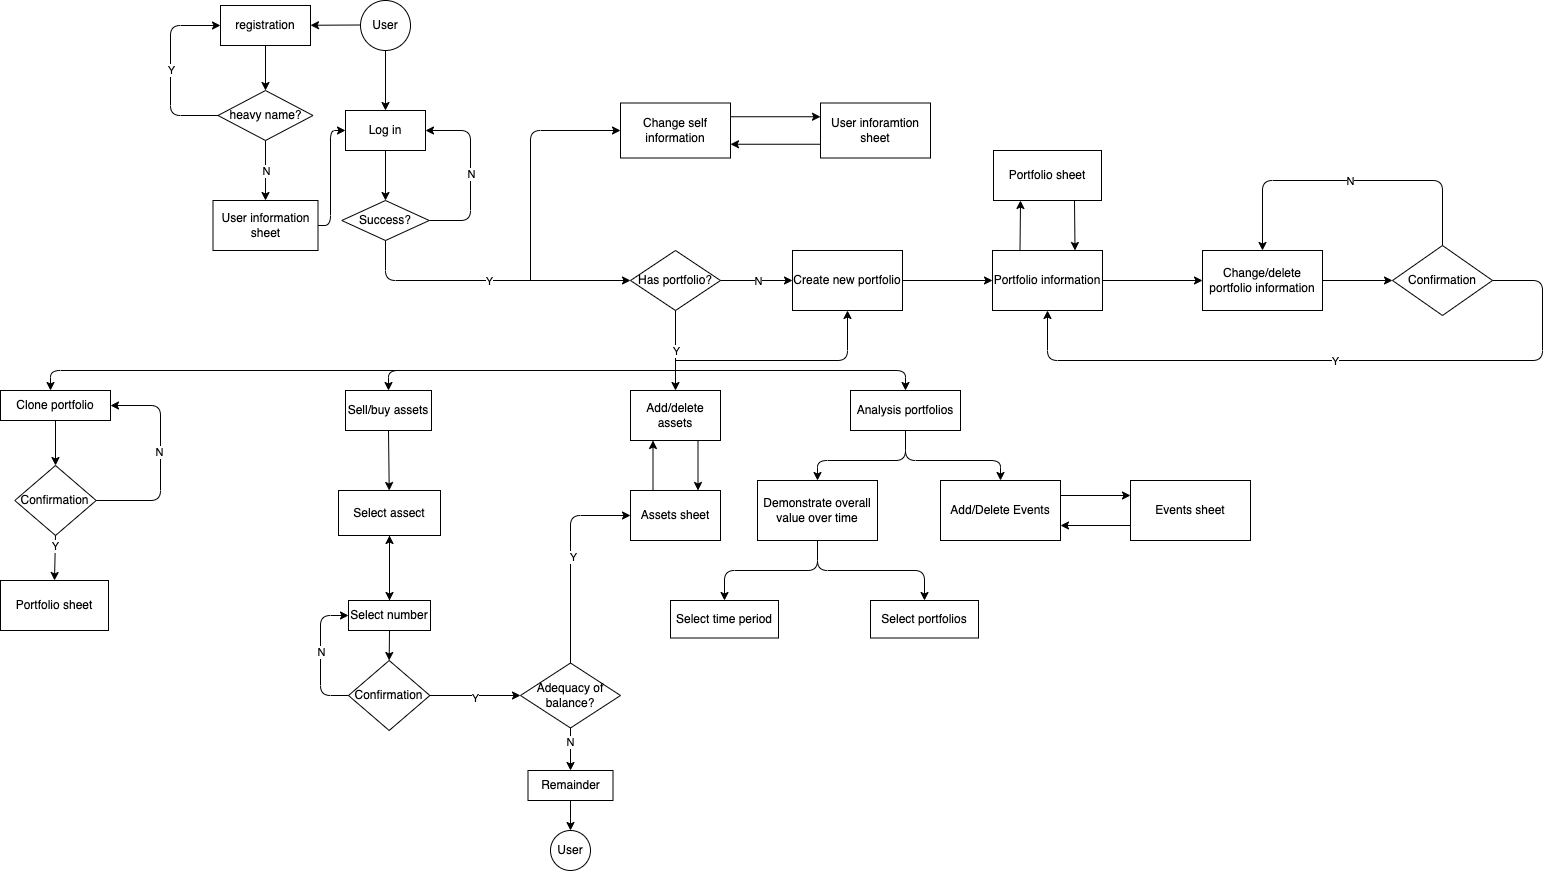
\includegraphics[width=0.8\textwidth]{../analysises/bussness process/V1.0/analysisV1.0.png}
    \caption{Diagramme de processus métier}
    \label{fig:processusMetier}
\end{figure}
\newpage
\subsection{Diagramme de UML}
\begin{figure}[h]
    \centering
    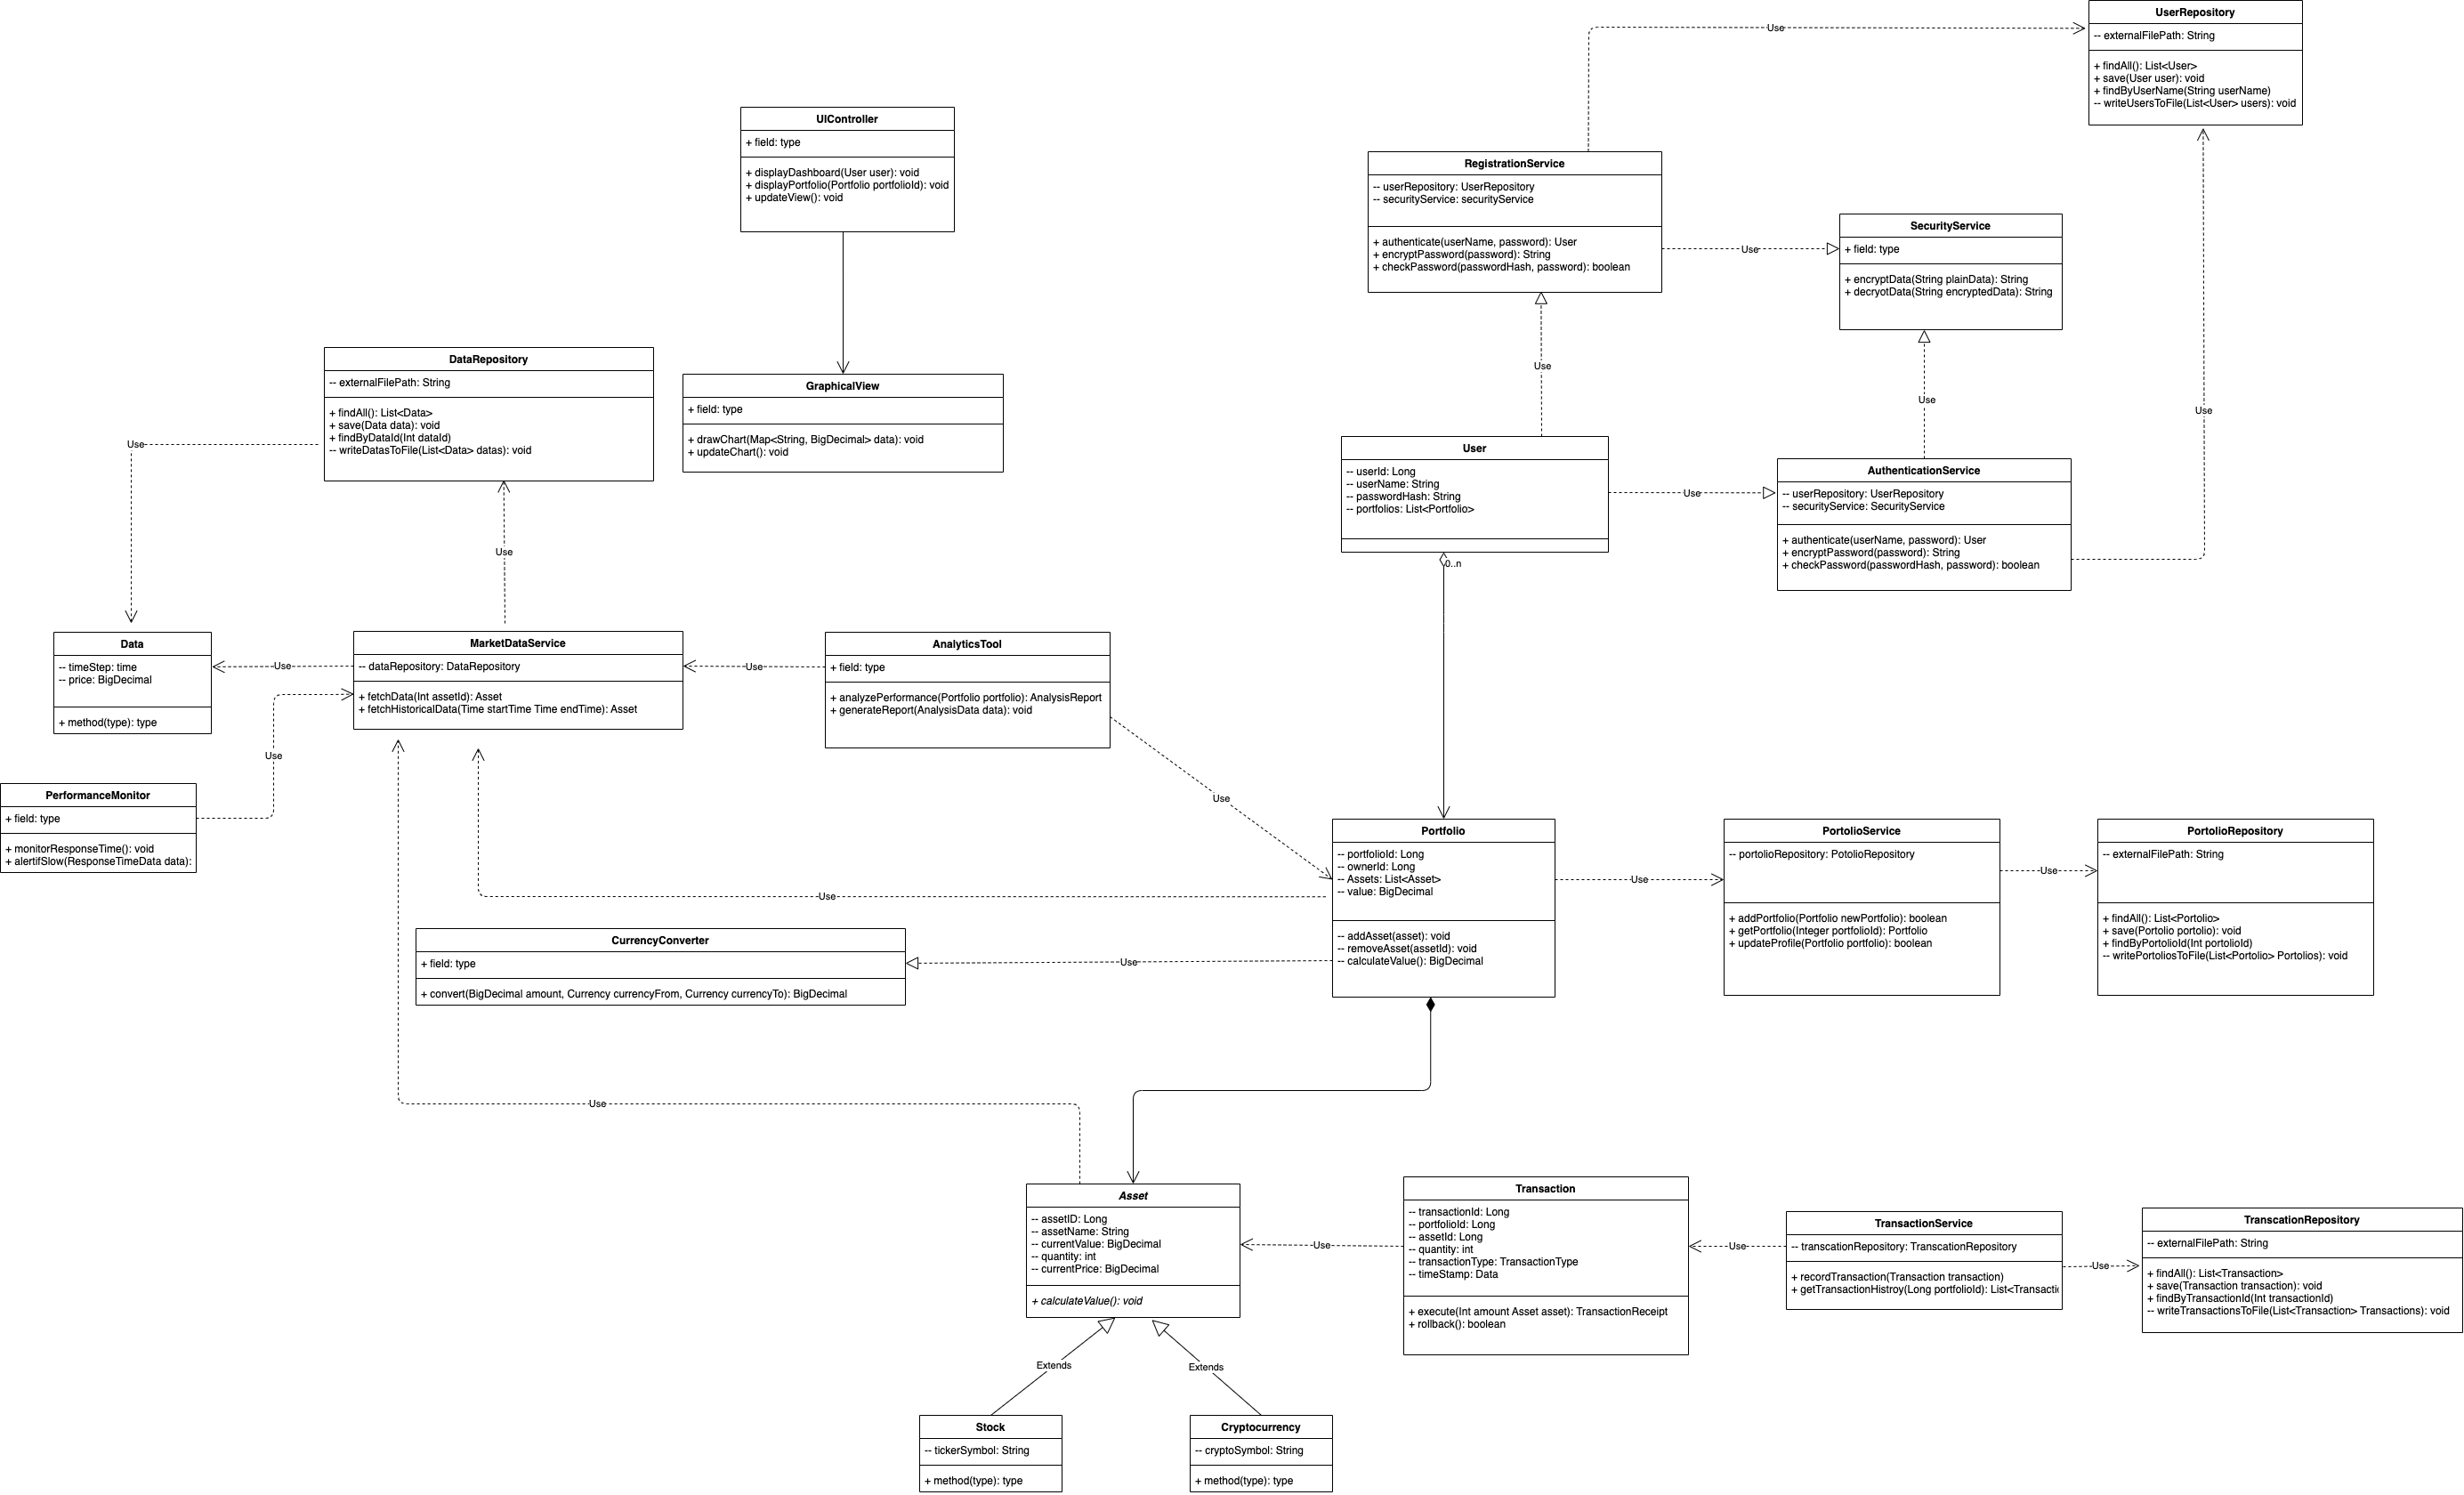
\includegraphics[width=0.8\textwidth]{../analysises/UML/V1.0/UMLV1.4.png}
    \caption{Diagramme de UML}
    \label{fig:UML}
\end{figure}

\subsection{Changement de Modèle de Conception}
\subsubsection{Introduction}




\section{Conception détaillée}
\subsection{Service}
\subsubsection{Registration Service (Service d'Enregistrement)}
\paragraph{Responsabilités:} Traite la logique d'enregistrement des nouveaux utilisateurs.
\paragraph{Méthodes:}
\begin{itemize}
  \item \textbf{register}(userName: String, password: String, passwordEnsurance: String): RegistrationResult
\end{itemize}
\paragraph{Exceptions:}
\begin{itemize}
  \item \textbf{IOException} : Si le fichier de stockage des utilisateurs n'est pas accessible. 
\end{itemize}
\subsubsection{Authentication Service (Service d'Authentification)}
\paragraph{Responsabilités:} Traite la logique d'authentification des utilisateurs.
\paragraph{Méthodes:}
\begin{itemize}
  \item \textbf{authenticate}(userName: String, password: String): AuthenticationResult
  \item \textbf{checkPassword}(passwordHash: String, password: String): Boolean
\end{itemize}
\subsubsection{Security Service (Service de Sécurité)}
\paragraph{Responsabilités:} Gère les opérations de sécurité et d'autorisation.
\paragraph{Méthodes:}
\begin{itemize}
  \item \textbf{encryptData}(plainData: String): String
  \item \textbf{decryptData}(encryptedData: String): String
\end{itemize}
\subsubsection{Portfolio Service (Service de Portefeuille)}
\paragraph{Responsabilités:} Gère les services de portefeuille d'investissement.
\paragraph{Méthodes:}
\begin{itemize}
  \item \textbf{getPortfolio}(portfolioId: int): Portfolio
  \item \textbf{updatePortfolio}(portfolio: Portfolio): Boolean
  \item \textbf{addPortfolio}(portfolio: Portfolio): Boolean
  \item \textbf{createPortfolio}(portfolioName : String, ownerId: int): Portfolio
\end{itemize}
\subsubsection{Asset Service (Service d'Actif)}
\paragraph{Responsabilités:} Gère les services d'actif.
\paragraph{Méthodes:}
\begin{itemize}
  \item \textbf{getAsset}(assetId: int): Asset
  \item \textbf{updateAsset}(asset: Asset): Boolean
  \item \textbf{addAsset}(asset: Asset): Boolean
  \item \textbf{createAsset}(assetName: String, portfolioId: int, quantity: int,
  price: BigDecimal, assetType: ASSET\_TYPE,  interestRate: BigDecimal): Asset
\end{itemize}

\subsubsection{Transaction Service (Service de Transaction)}
\paragraph{Responsabilités:} Gère la logique des transactions.
\paragraph{Méthodes:}
\begin{itemize}
  \item \textbf{recordTransaction}(transaction: Transaction): void
  \item \textbf{getTransactionHistory}(portfolioId: int): List<Transaction>
\end{itemize}
\subsubsection{Market Data Service (Service des Données du Marché)}
\paragraph{Responsabilités:} Fournit des services de données de marché.
\paragraph{Méthodes:}
\begin{itemize}
  \item \textbf{fetchData}(assetId: int): List<Asset>
  \item \textbf{fetchHistoricalData}(startTime: Time, endTime: Time): List<Asset>
\end{itemize}
\paragraph{Exceptions:}
\begin{itemize}
  \item \textbf{IOException} : Si l'API externe est inaccessible.
\end{itemize}
\subsection{Repository}
\subsubsection{User Repository (Dépôt Utilisateur)}
\paragraph{Responsabilités:} Gère le stockage et la récupération des données utilisateur.
\paragraph{Méthodes:}
\begin{itemize}
  \item \textbf{findAll}(): List<User>
  \item \textbf{save}(user: User): Boolean
  \item \textbf{findByUserName}(userName: String): User
\end{itemize}

\subsubsection{Data Repository (Dépôt de Données)}
\paragraph{Responsabilités:} Gère le stockage et la récupération des données d'application.
\paragraph{Méthodes:}
\begin{itemize}
  \item \textbf{findAll}(): List<Asset>
  \item \textbf{save}(Data: data): Boolean
  \item \textbf{findByDataTimeStamp}(dataTimeStamp: Time): Data
  \item \textbf{findByDataTimeStamp}(startTime: Time, endTime: Time): List<Data>
\end{itemize}
\subsubsection{Transaction Repository (Dépôt de Transaction)}
\paragraph{Responsabilités:} Gère le stockage et la récupération des données de transaction.
\paragraph{Méthodes:}
\begin{itemize}
  \item \textbf{findAll}(): List<Transaction>
  \item \textbf{save}(transaction: Transaction): Boolean
  \item \textbf{findByPortfolioId}(portfolioId: int): List<Transaction>
\end{itemize}
\subsubsection{Portfolio Repository (Dépôt de Portefeuille)}
\paragraph{Responsabilités:} Gère le stockage et la récupération des données de portefeuille d'investissement.
\paragraph{Méthodes:}
\begin{itemize}
  \item \textbf{findAll}(): List<Portfolio>
  \item \textbf{save}(portfolio: Portfolio): Boolean
  \item \textbf{findByPortfolioId}(portfolioId: int): Portfolio
\end{itemize}
\subsubsection{Asset Repository (Dépôt d'Actif)}
\paragraph{Responsabilités:} Gère le stockage et la récupération des données d'actif.
\paragraph{Méthodes:}
\begin{itemize}
  \item \textbf{findAll}(): List<Asset>
  \item \textbf{save}(asset: Asset): Boolean
  \item \textbf{findByAssetId}(assetId: int): Asset
  \item \textbf{findByOwnerId}(ownerId: int): List<Asset>
\end{itemize}
\subsection{Model}
\subsubsection{Analytics Tool (Outil d'Analyse)}
\paragraph{Responsabilités:} Fournit des outils d'analyse de données.
\subsubsection{Performance Monitor (Surveillance de la Performance)}
\paragraph{Responsabilités:} Surveille la performance du Service des Données du Marché pour déterminer si l'API externe est trop lente.
\subsubsection{User (Utilisateur)}
\paragraph{Responsabilités:} Représente un utilisateur.
\paragraph{Propriétés:}
\begin{itemize}
  \item \textbf{userName}: String
  \item \textbf{userId}: int
  \item \textbf{passwordHash}: String
  \item \textbf{portfolios}: List<Portfolio>
\end{itemize}
\subsubsection{Data (Donnée)}
\paragraph{Responsabilités:} Représente une donnée collecté.
\paragraph{Propriétés:}
\begin{itemize}
  \item \textbf{price}: BigDecimal
  \item \textbf{timeStamp}: Time
\end{itemize}
\subsubsection{Authentication Result (Résultat d'Authentification)}
\paragraph{Responsabilités:} Représente le résultat d'une tentative d'authentification.
\paragraph{Propriétés:}
\begin{itemize}
  \item \textbf{sucess}: Boolean
  \item \textbf{failureType}: AUTHENTICATION\_FAILIURE\_TYPE
  \item \textbf{user}: User
\end{itemize}
\subsubsection{Registration Result (Résultat d'Inscription)}
\paragraph{Responsabilités:} Représente le résultat d'une tentative d'inscription.
\paragraph{Propriétés:}
\begin{itemize}
  \item \textbf{sucess}: Boolean
  \item \textbf{failureType}: REGISTRATION\_FAILIURE\_TYPE
  \item \textbf{user}: User
\end{itemize}
\subsubsection{Portfolio (Portefeuille)}
\paragraph{Responsabilités:} Représente un portefeuille d'investissement.
\paragraph{Propriétés:}
\begin{itemize}
  \item \textbf{portfolioId}: int
  \item \textbf{ownerId}: int
  \item \textbf{assets}: List<Asset>
\end{itemize}
\subsubsection{Asset (Actif)}
\paragraph{Responsabilités:} Représente un actif.
\paragraph{Propriétés:}
\begin{itemize}
  \item \textbf{assetId}: int
  \item \textbf{assetName}: String
  \item \textbf{assetType}: ASSET\_TYPE
  \item \textbf{quantity}: int
  \item \textbf{price}: BigDecimal
  \item \textbf{value}: BigDecimal
\end{itemize}
\subsubsection{Transaction (Transaction)}
\paragraph{Responsabilités:} Représente une transaction.
\paragraph{Propriétés:}
\begin{itemize}
  \item \textbf{transactionId}: int
  \item \textbf{portfolioId}: int
  \item \textbf{assetId}: int
  \item \textbf{quantity}: int
  \item \textbf{transactionType}: TRANSACTION\_TYPE
  \item \textbf{timeStamp}: Time
\end{itemize}
\section{Guide de développement et de déploiement}
\section{Test Plan et Test Cases}
\section{Manuel de l'utilisateur}
\section{Évaluation des performances}
\section{Exemple de code}
\section{Journal des modifications}
\section{Annexe}
\end{document}